% ---------------------------------------------------------------------------
\section{Introduction}
\label{sec:intro}

Panoramic dental radiograph analysis requires assigning diagnostic findings to individual
teeth in standard FDI notation. General-purpose vision-language models (VLMs) offer a flexible
interface, but our zero-shot evaluation on DENTEX shows limited finding-level agreement with
expert annotations (\cref{sec:baselines}). The best reported pooled exact F1 is 0.222.
Image-level hit rates and calibration provide complementary evidence, but do not by themselves
identify the causes of these errors. Local detail, tooth identity, and orientation motivate an
agent that can inspect a region again before answering.

Medical and general-purpose tool-using systems provide relevant precedents
\citep{wu2026vtool,li2024mmedagent,zhang2025octotools,oralgptplus2026,oralagent2026}.
We focus on a specific failure point: a learned grounding model can return a plausible box for
the wrong region, and subsequent crops inherit that error. Rather than treating the box as an
authoritative observation, the policy should be able to inspect and revise it. Whether a
trained policy acquires this behavior, and whether it improves diagnosis, are empirical
questions addressed by the frozen evaluation design.

This paper develops and evaluates \sys{}, an agentic VLM for OPG diagnosis built around a
different contract between the policy and its tools: \emph{grounding is a hypothesis, not an
answer} (\cref{fig:concept}). \cref{fig:architecture,fig:training} give the complete system architecture (agent loop and offline
training stack), and \cref{fig:evidence,fig:traces} contrast the two trace arms on one image. Our contributions are:

\begin{figure}[tbp]
  \centering
  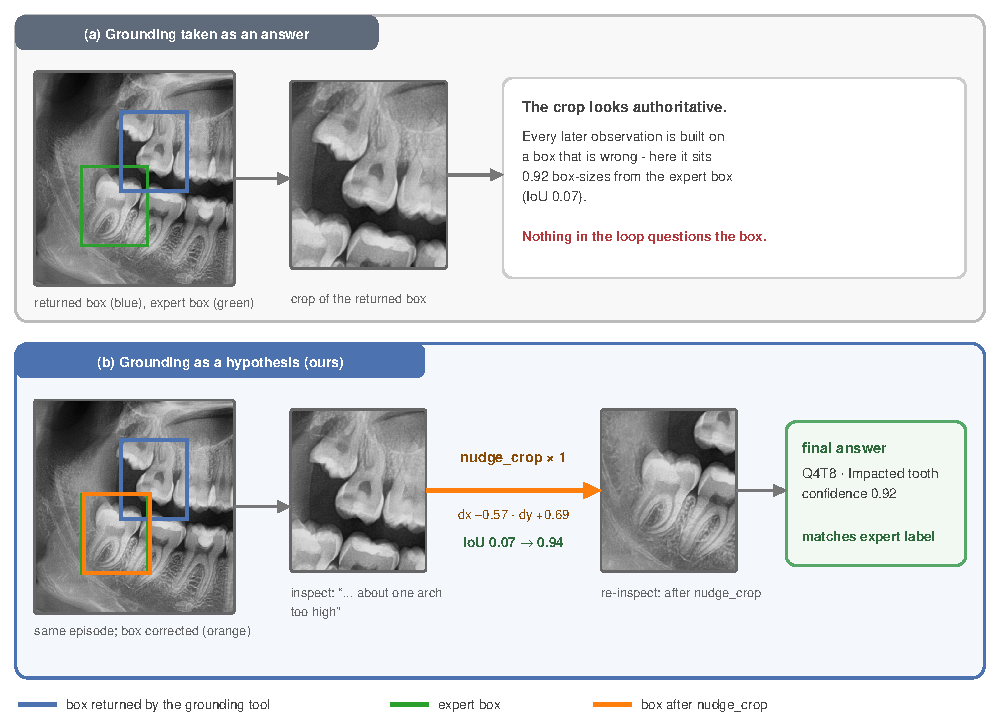
\includegraphics[width=\linewidth]{fig_concept}
  \caption{The central idea, on a real episode from the corpus (DENTEX image 127, an impacted FDI
  tooth 48). (a) When a grounding box is taken as an answer, the crop of that box looks
  authoritative and every later observation inherits its error --- here the returned box (blue)
  sits 0.92 box-sizes from the expert box (green; IoU 0.07). (b) \sys{} treats the box as a
  hypothesis: the policy sees a crop dominated by an upper molar, judges the box ``about one arch
  too high'', corrects it with one box-relative \texttt{nudge\_crop} (orange; IoU 0.94), and
  answers from the corrected view. Crops are native-resolution views of the box with 30\% padding, illustrative of what the zoom
  tool returns rather than the canonical-view geometry of \cref{fig:inputgeom}. Further episodes
  are in \cref{fig:gallery}; the full with-tools trace of another image is dissected in
  \cref{fig:evidence,fig:traces}.}
  \label{fig:concept}
\end{figure}

\begin{enumerate}[leftmargin=*,itemsep=2pt,topsep=3pt]
\item \textbf{A self-correcting grounding tool (\texttt{nudge\_crop}, \cref{sec:nudge}).}
The policy can shift and rescale a box it was \emph{already given} --- by the grounding model or
by a previous correction --- using box-relative fractional arguments (\texttt{dx\_frac},
\texttt{dy\_frac}, \texttt{scale}) that a VLM can reason about linguistically
(``shift right about half a tooth-width''), without re-running detection. We make box revision an explicit, inspectable action rather than an implicit change in the
policy's internal localization.
\item \textbf{A tiered perturbation mechanism that makes self-correction learnable
(\cref{sec:perturbation}).} Demonstrating correction behavior requires the demonstrator to
\emph{experience} tool error. During trace generation we return the expert-verified box for
annotated teeth (guaranteeing task solvability) but deliberately perturb the box
\emph{shown to the demonstrator} --- 45\% clean, 25\% small offsets (12--28\% of box size), 30\%
large offsets (45--75\%) --- with two design commitments: the rates are fixed constants decoupled
from the detector's real error rate, so demonstrations never go stale as the detector improves;
and errors are never announced verbally, so correction must be elicited by the returned image rather than an explicit error message.
Transfer of this behavior to the trained policy remains to be measured. A corpus-level analysis (\cref{sec:mechanism}) shows the mechanism elicits exactly the
intended behavior gradient in 3{,}694 generated demonstrations: corrective use of
\texttt{nudge\_crop} on 38.4\% of large offsets, 13.6\% of small ones (intermediate offsets),
and 1.1\% of clean boxes, on ground-truth-anchored pathology locates.
\item \textbf{A tool interface with continuous parameters (\cref{sec:tools}).} Tools expose
\emph{how much} effect to apply, not just which tool to call: \texttt{denoise(strength
$\in[0,1]$)}, \texttt{window\_level} with exact \texttt{center}/\texttt{width} values as an
override on top of presets, a multiplicative \texttt{enhance\_contrast} factor, and a tunable
\texttt{zoom\_crop} context margin. Tool calls therefore
carry real information beyond tool identity, and the policy can match processing intensity to
image characteristics.
\item \textbf{A ground-truth-anchored, correction-friendly reward (\cref{sec:reward}).} GRPO
training \citep{deepseek2025r1} uses a composite reward whose dominant term is a hard,
non-LLM-judge match against expert labels with multi-finding greedy one-to-one matching
(F1-style harmonic mean of recall and precision), and whose efficiency term scales a reference
budget with case complexity and \emph{exempts} \texttt{locate\_tooth} and \texttt{nudge\_crop}
from per-call cost --- so the reward never prices out the verification behavior it is trying to
teach, a failure mode we identified and removed by design.
\item \textbf{Label-anchored synthetic demonstrations and an audit trail
(\cref{sec:traces}).} 3{,}694 verified chain-of-thought tool-use traces over DENTEX and Tufts
(1{,}847 with tools, 1{,}847 single-turn without, exact 1:1 parity), generated by frontier models
under real tool execution in a LangGraph loop, verified cross-family, decontaminated of
directive leakage (105 traces regenerated; 0 leaks in the canonical corpus), and released as a
reusable resource. The verifier's rejection taxonomy (66 false-positive findings on healthy
scans, 15 ground-truth contradictions, 11 uncorrected spatial drifts) doubles as an audit of
what the perturbation mechanism does and does not elicit.
\end{enumerate}

We evaluate on DENTEX with its native structured metrics --- pooled, set-matched,
finding-level precision/recall/F1 with paired bootstrap intervals --- against zero-shot frontier
VLMs, the same backbone with and without tools, and a supervised specialist detector. The
training-side analyses in this draft are complete; the two-stage training runs (SFT, then GRPO)
are not yet reported, and their result cells are marked \todo{SFT/GRPO results pending first
hardware run} rather than extrapolated. Inference-time rules, skills, and serving optimizations are evaluated
separately on the training-derived dev split (\cref{sec:harness-serving}); they do not revise
the frozen primary protocol.
